\section{Linux Platform / Devkit 8000 Applikationsmodel}

\subsection{Applikationsmodel usecase 1}
\begin{figure}[H]
\caption{Sekvensdiagram usecase 1: åbn vinflaske på devkit 8000}
\label{SD:UC1-devkit}
\includegraphics[scale=0.4,trim=0 0 350 0, clip]{SD-åbn-vinflaske-Linux-platform}
\end{figure}

På figur \ref{CD:UC1-devkit} side \pageref{CD:UC1-devkit} ses det resulterende klassediagram efter metodeidentifikation udført på basis af sekvensdiagrammet på figur \ref{SD:UC1-devkit} side \pageref{SD:UC1-devkit}.
\begin{figure}[H]
	\caption{Klassediagram usecase 1: åbn vinflaske på devkit 8000}
	\label{CD:UC1-devkit}
	\includegraphics[scale=0.35]{CD-åbn-vinflaske-Linux-platform}
\end{figure}

\subsection{Applikationsmodel usecase 2}

Enkelte ekstensions er udeladt på sekvensdiagrammet da de blot resultere i en terminering af usecase sekvensen.

\begin{figure}[H]
	\caption{Sekvensdiagram usecase 2: Planlæg åbning på devkit 8000}
	\label{SD:UC2-devkit}
	\includegraphics[scale=0.4]{SD-planlaeg-åbning-Linux-platform}
\end{figure}

På figur \ref{CD:UC2-devkit} side \pageref{CD:UC2-devkit} ses det resulterende klassediagram efter metodeidentifikation udført på basis af sekvensdiagrammet på figur \ref{SD:UC2-devkit} side \pageref{SD:UC2-devkit}.
\begin{figure}[H]
	\caption{Klassediagram usecase 2: Planlæg åbning på devkit 8000}
	\label{CD:UC2-devkit}
	\includegraphics[scale=0.35]{CD-planlaeg-åbning-Linux-platform}
\end{figure}

\subsection{Applikationsmodel usecase 3}

\begin{figure}[H]
	\caption{Sekvensdiagram usecase 3: Indstil tid på devkit 8000}
	\label{SD:UC3-devkit}
	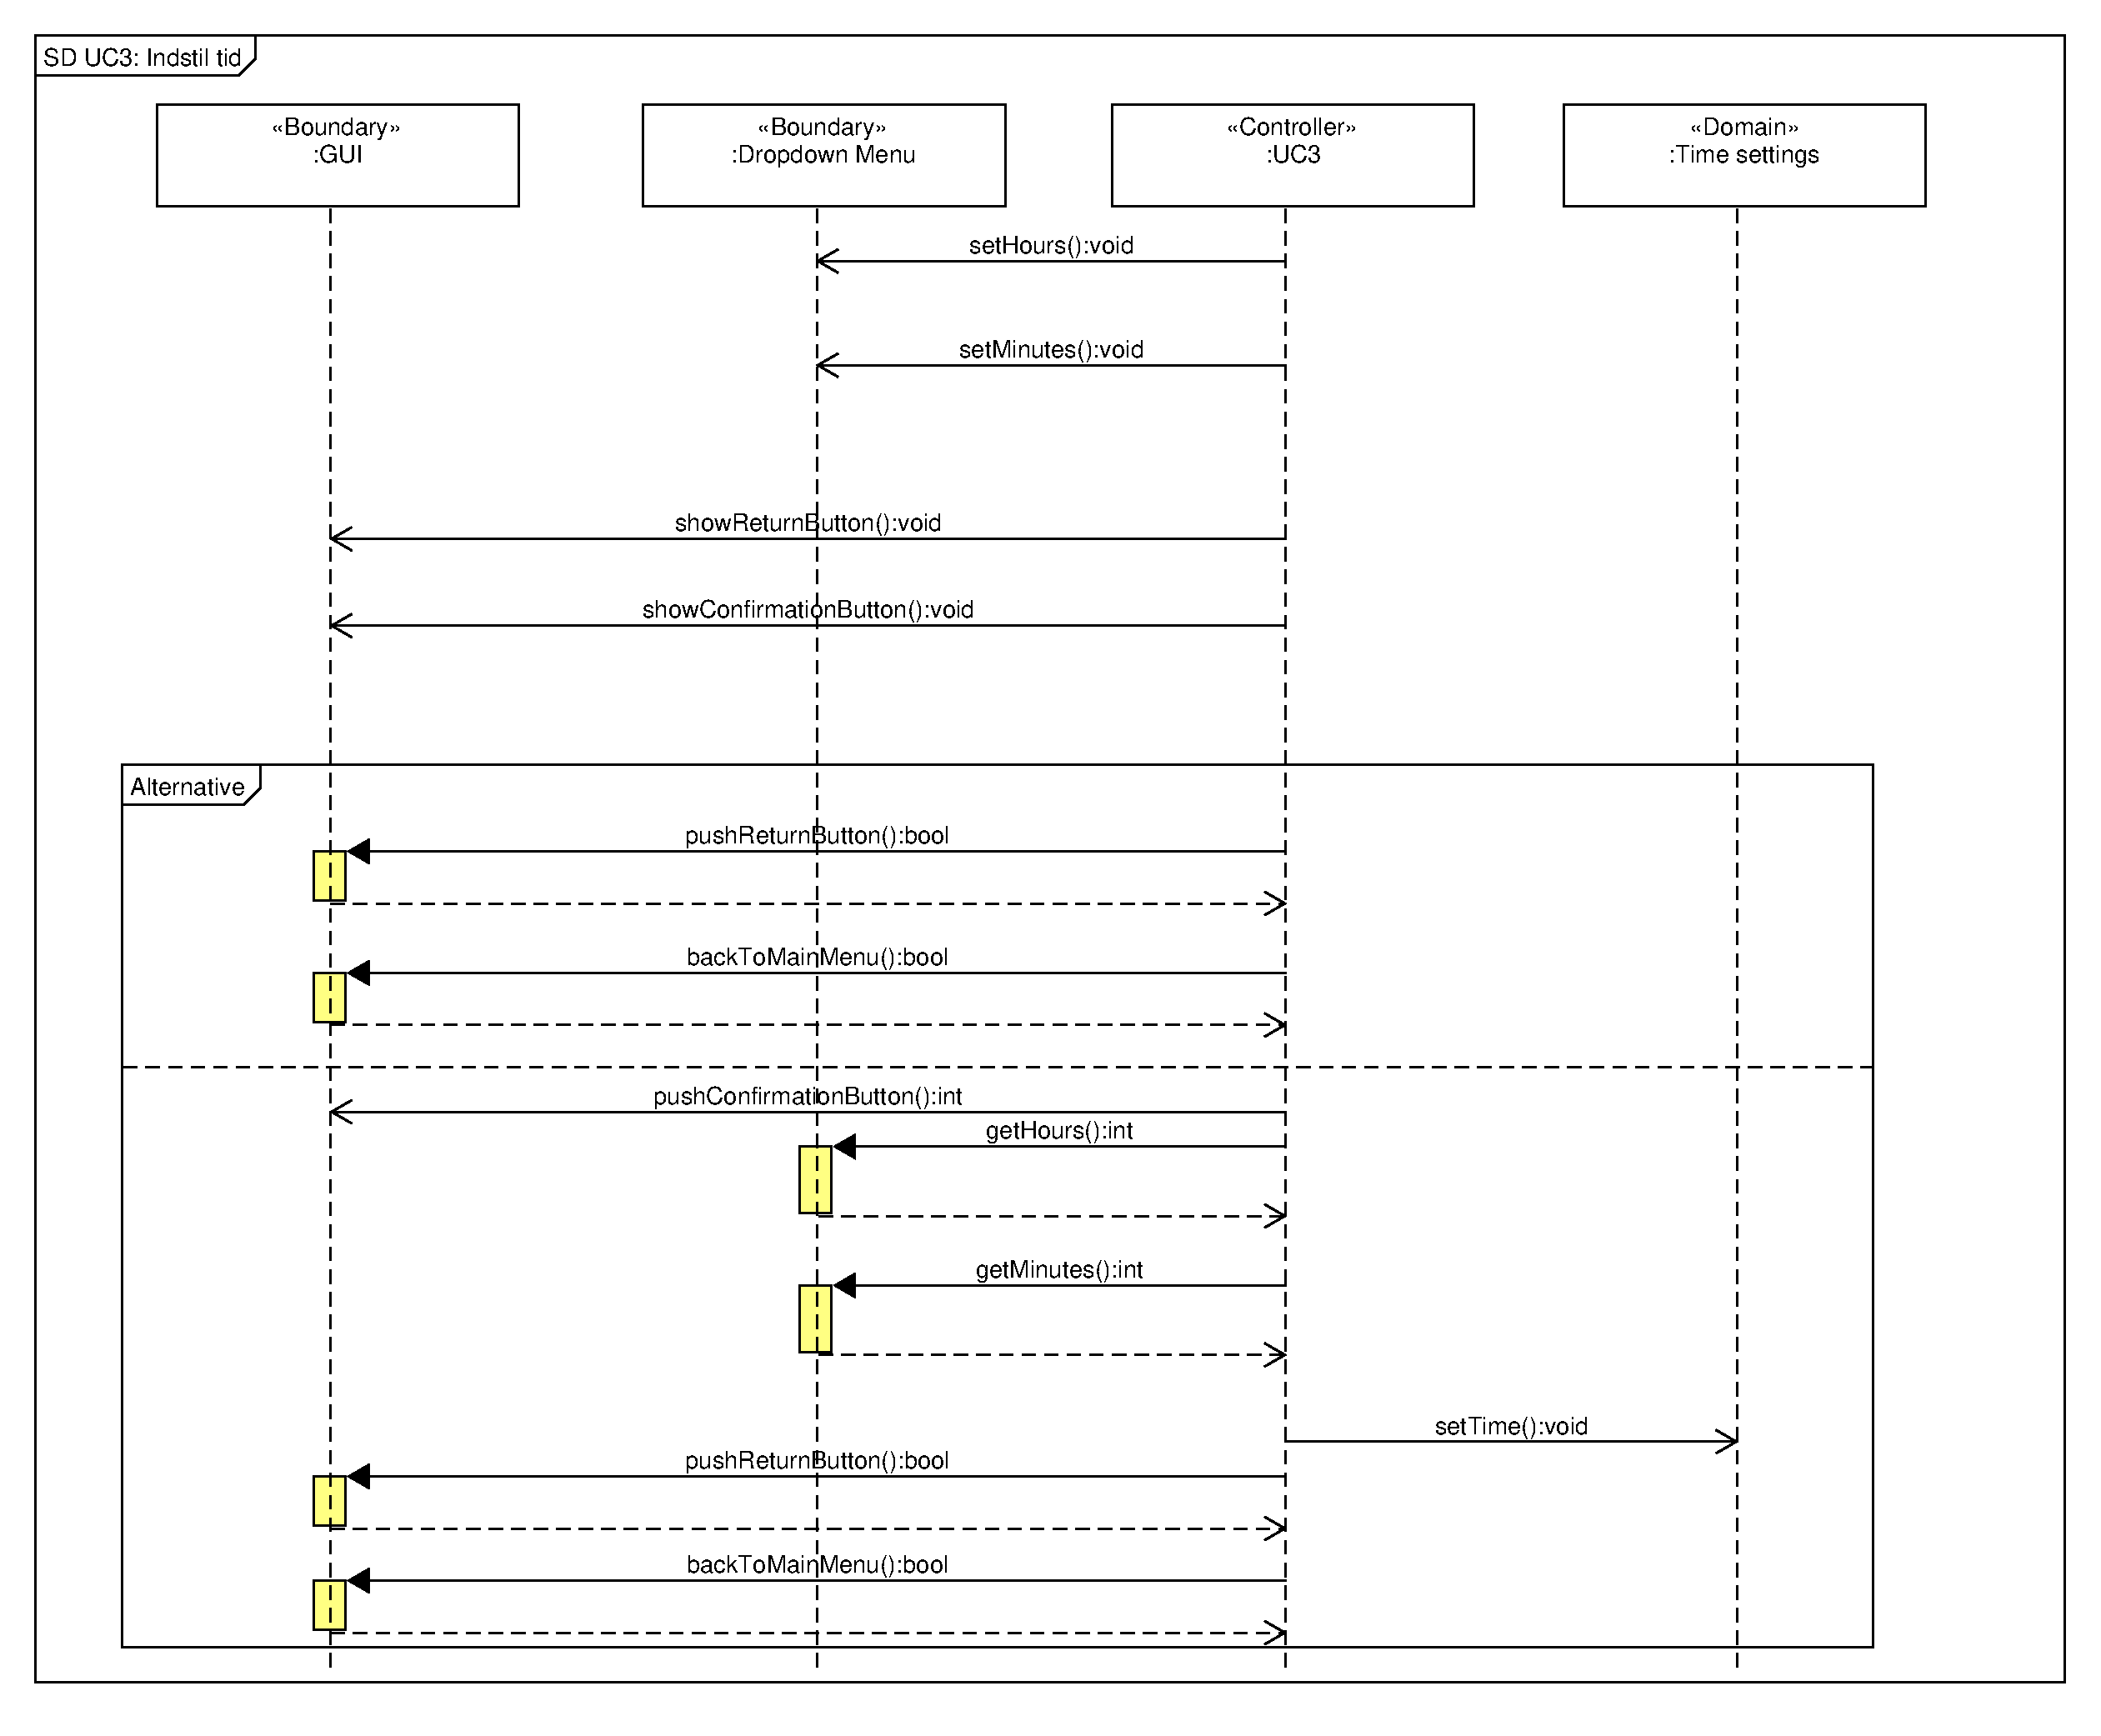
\includegraphics[scale=0.6,trim=10 400 100 0]{Applikationsmodel_UC3/SD_UC3}
\end{figure}

\begin{figure}[H]
	\caption{Statemachine Diagram usecase 3: Indstil tid på devkit 8000}
	\label{STD:UC3-devkit}
	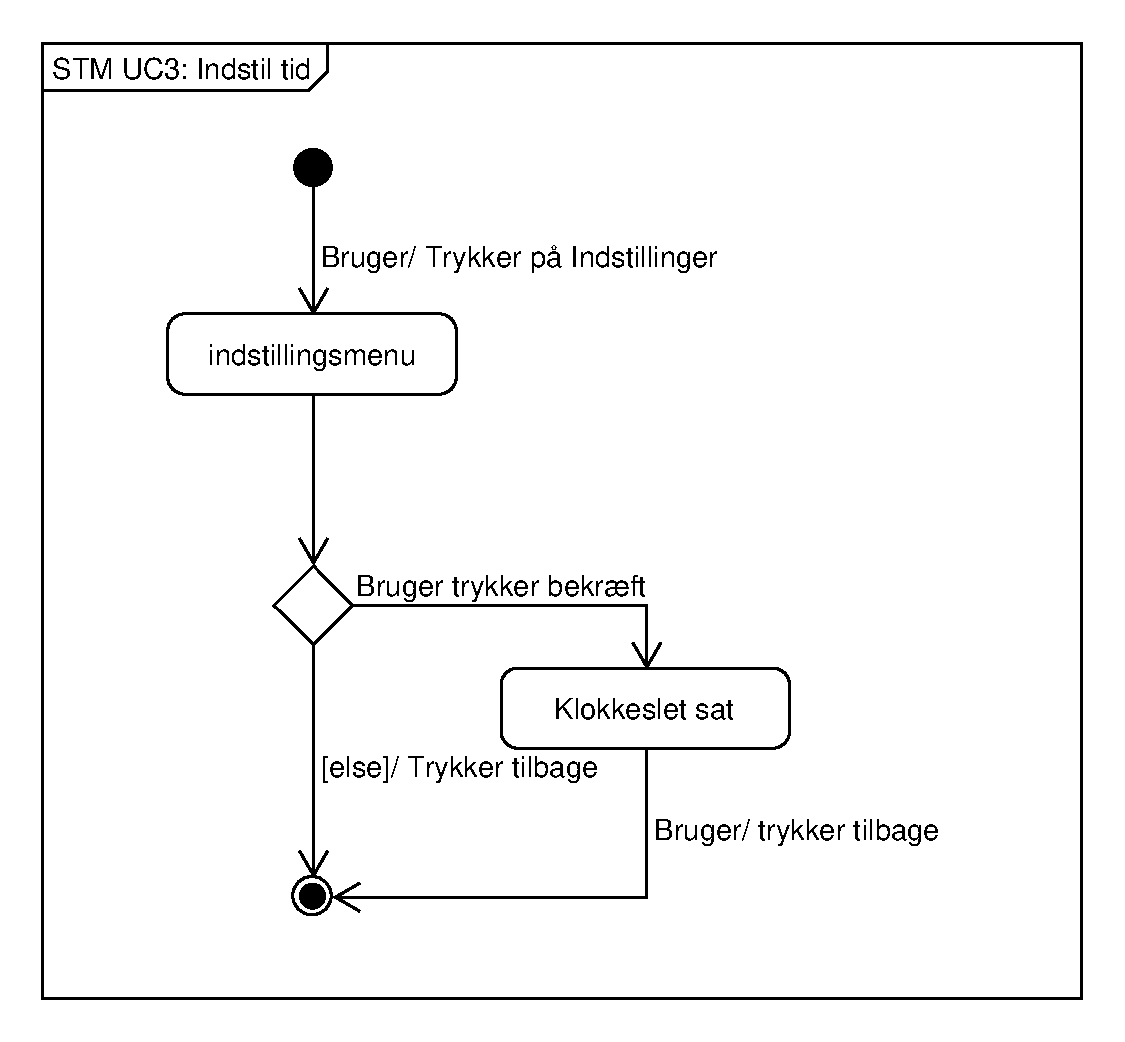
\includegraphics[scale=0.7,trim=10 600 100 0, clip]{Applikationsmodel_UC3/Statemachine_UC3}
\end{figure}

På figur \ref{CD:UC3-devkit} side \pageref{CD:UC3-devkit} ses det resulterende klassediagram efter metodeidentifikation udført på basis af sekvensdiagrammet på figur \ref{SD:UC3-devkit} side \pageref{SD:UC3-devkit}.
\begin{figure}[H]
	\caption{Klassediagram usecase 3: Indstil tid på devkit 8000}
	\label{CD:UC3-devkit}
	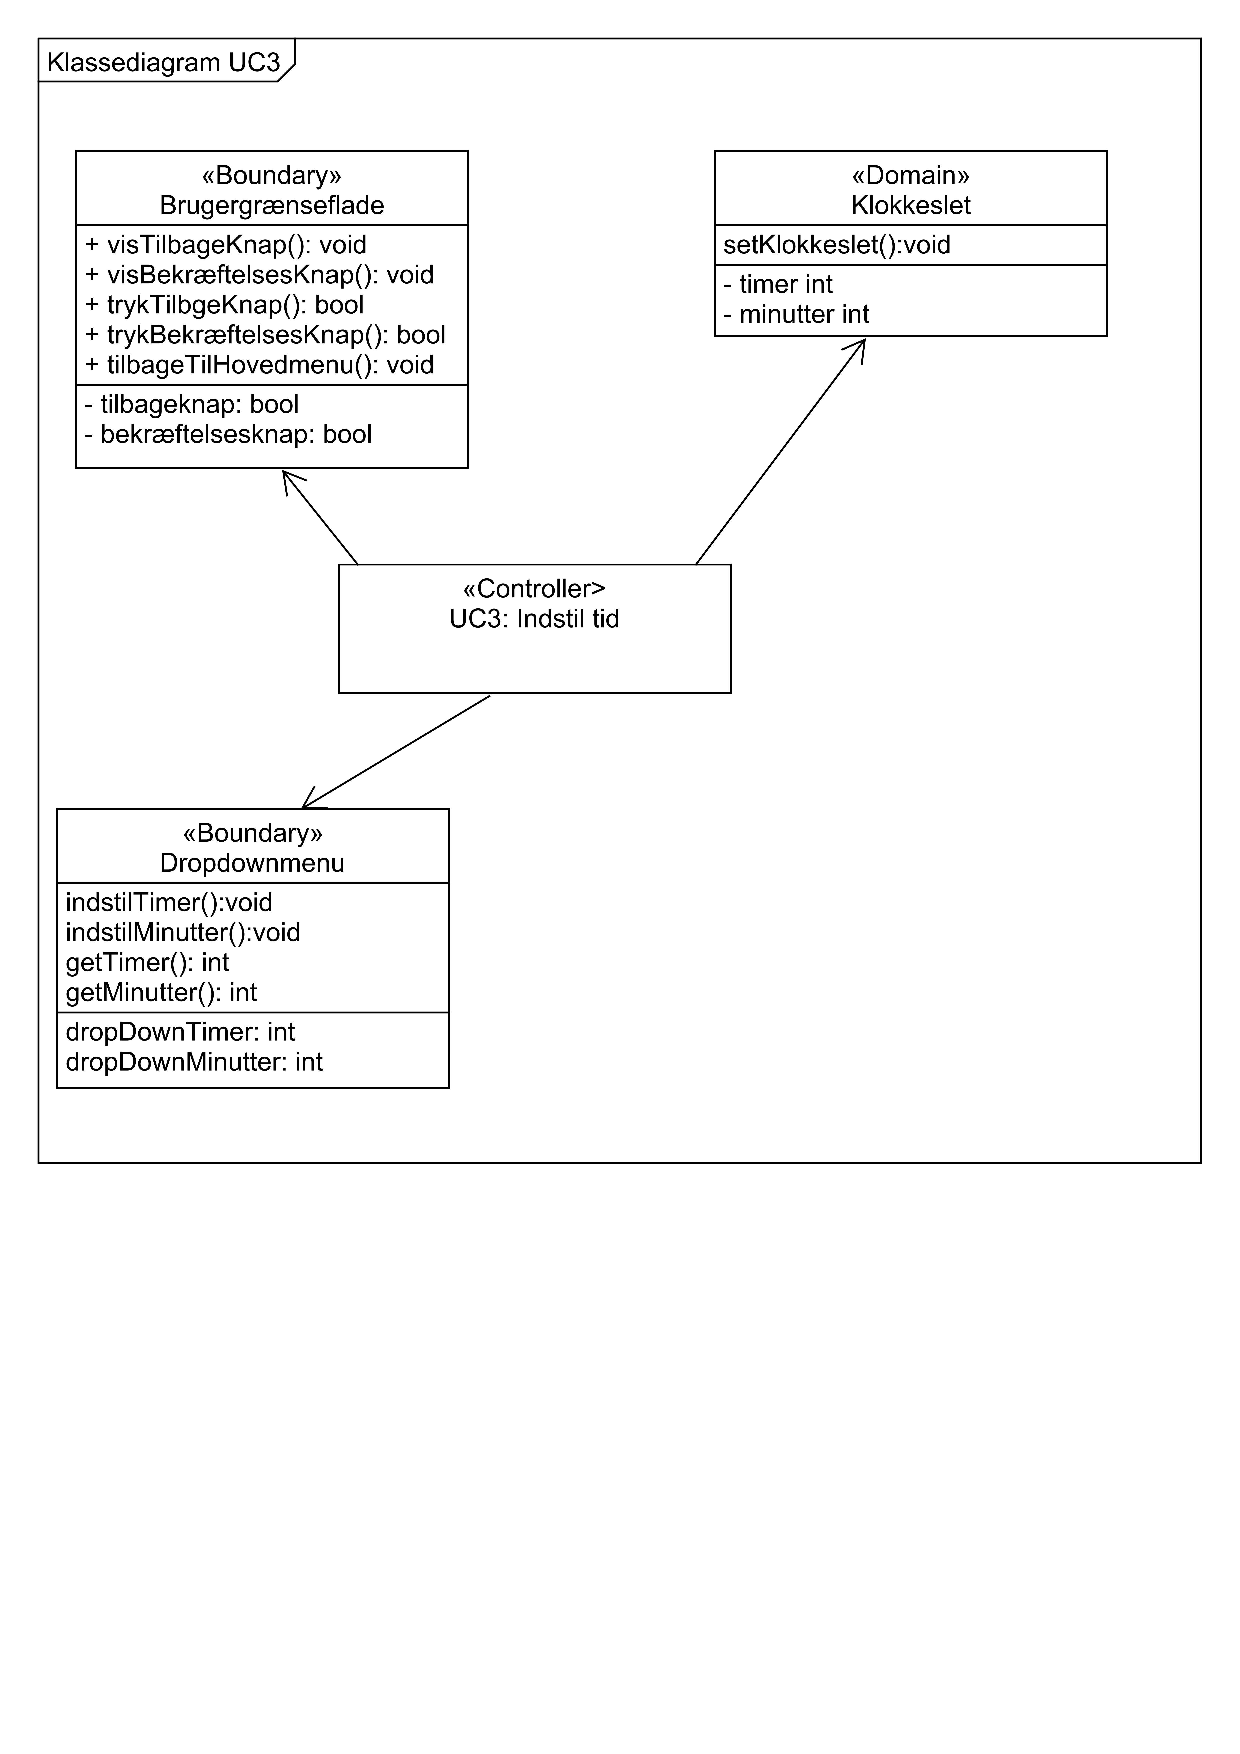
\includegraphics[scale=0.6,trim=10 800 100 0]{Applikationsmodel_UC3/Klassediagram_UC3.pdf}
\end{figure}
